\chapter{PHÂN TÍCH HỆ THỐNG}\label{ch:analysis}

\section{Phương pháp phân tích hướng đối tượng}
Phân tích hệ thống áp dụng cách tiếp cận hướng đối tượng dẫn dắt bởi use case.\allowbreak{} Từ mục tiêu và hành động của tác nhân, xác định các đối tượng lĩnh vực, trách nhiệm và vòng đời.\allowbreak{} Các mô hình tương tác làm rõ cách phối hợp giữa đối tượng trước khi xác định cấu trúc thành phần ở mức thiết kế.\allowbreak{}

Mức phân tích không cần mô tả từng hàm PHP.\allowbreak{} Ví dụ, tác nhân yêu cầu đặt lịch, đối tượng điều khiển kiểm tra giờ và ghi lịch, các thực thể là Bệnh nhân, Bác sĩ, Ca khám và Lịch hẹn.\allowbreak{} Mức thiết kế mới nêu Appointment\allowbreak{}Booking\allowbreak{}Service và DB:\allowbreak{}:\allowbreak{}transaction.\allowbreak{}

Mô hình biên-điều khiển-thực thể (BCE) phân chia trách nhiệm thành ba nhóm.\allowbreak{} Lớp biên tiếp nhận và trình bày thông tin; lớp điều khiển điều phối kịch bản, kiểm tra điều kiện và quản lý giao dịch; lớp thực thể biểu diễn dữ liệu nghiệp vụ có vòng đời dài hạn.\allowbreak{} Sự phân chia này giúp giảm phụ thuộc giữa giao diện và quy tắc xử lý.\allowbreak{}

UML là ngôn ngữ mô tả mô hình; sơ đồ trong báo cáo được chọn theo câu hỏi cần trả lời.\allowbreak{} Use case mô tả mục tiêu bên ngoài, activity mô tả nhánh quy trình, sequence mô tả thứ tự trao đổi, state mô tả vòng đời và ERD mô tả lược đồ lưu trữ.\allowbreak{} Một sơ đồ không thay thế tất cả góc nhìn còn lại.\allowbreak{}


\section{Phân biệt danh tính, hồ sơ và lần khám}
User là danh tính xác thực, Patient là hồ sơ hành chính và y tế nền, Visit là một lần phục vụ cụ thể.\allowbreak{} Ba khái niệm có vòng đời khác nhau.\allowbreak{} Một người vãng lai có thể có Patient mà không có User; khóa tài khoản không xóa hồ sơ hoặc các chứng từ khám trước.\allowbreak{}

Doctor là hồ sơ chuyên môn gắn một User.\allowbreak{} Vai trò doctor không thay cho phân công cơ sở; thuộc tính chuyên khoa chính không thay cho bảng quan hệ các chuyên khoa bổ sung.\allowbreak{} Ca, nghỉ và lượt sử dụng doctor\_\allowbreak{}id để kiểm tra bận và trách nhiệm điều trị.\allowbreak{}

Appointment chứa ý định tương lai và có thể kết thúc ở CANCELLED/\allowbreak{}NO\_\allowbreak{}SHOW mà không có Visit.\allowbreak{} Khi check-in thành công, Visit được tạo một lần.\allowbreak{} Vì vậy dùng một bảng duy nhất cho cả hẹn và khám sẽ làm khó mô tả khách vãng lai và điều kiện ký hồ sơ.\allowbreak{}

Các quan hệ tùy chọn phản ánh vòng đời nghiệp vụ:\allowbreak{} lượt vãng lai có thể không có lịch hẹn; bệnh nhân có thể chưa đăng ký tài khoản; hồ sơ khám hiện hành luôn thuộc một lượt.\allowbreak{} Bội số của quan hệ được xác định bằng điều kiện bắt buộc và tính duy nhất, sau đó được bảo vệ bằng khóa ngoại, chỉ mục và kiểm tra nghiệp vụ.\allowbreak{}


\section{Ranh giới nhất quán và các đối tượng gốc}
Nhóm lịch đặt lấy bác sĩ làm điểm khóa điều phối vì mọi ca, nghỉ và thay đổi lịch đều có thể ảnh hưởng khả dụng của cùng người khám.\allowbreak{} Khi đặt/\allowbreak{}đổi còn khóa bệnh nhân để chặn hai lịch trùng do hai bác sĩ khác nhau cùng được chọn đồng thời.\allowbreak{}

Nhóm khám lấy Visit làm gốc kiểm điều kiện.\allowbreak{} Hồ sơ, đơn và chỉ định chỉ thay đổi khi trạng thái Visit cho phép.\allowbreak{} Nhóm tài chính tách điểm chốt giá ở phát hành Invoice và điểm số dư ở Payment/\allowbreak{}Refund; khóa Invoice bảo vệ phép kiểm còn phải thu.\allowbreak{}

Nhóm kho khóa Prescription để bảo vệ số lượng còn được cấp, rồi khóa lô theo trật tự và giảm tồn có điều kiện.\allowbreak{} Lịch nhân viên dùng khóa điều phối và fingerprint tập phương án khi chốt.\allowbreak{} Bảng lương khóa user và entry đồng thời dùng version.\allowbreak{}

Mỗi ranh giới nhất quán xác định tập dữ liệu cần kiểm tra và cập nhật trong cùng một giao dịch.\allowbreak{} Khi giao dịch thất bại, toàn bộ thay đổi trong phạm vi đó được hoàn tác.\allowbreak{} Cách tổ chức này bảo vệ các bất biến về chỗ khám, số dư, số lượng thuốc và trạng thái lịch nhân sự khi nhiều người thao tác đồng thời.\allowbreak{}


\section{Phân tích lớp biên, điều khiển và thực thể}
Lớp biên gồm các trang Blade, form và đoạn Java\allowbreak{}Script tải slot/\allowbreak{}ca.\allowbreak{} Controller nhận dữ liệu HTTP, validate và chọn response.\allowbreak{} Với màn hình lịch tuần, boundary chỉ hiển thị các ca, khi nhấn một ca mới yêu cầu danh sách bệnh nhân.\allowbreak{} Thiết kế giảm lượng thông tin nhạy cảm xuất hiện trước nhu cầu.\allowbreak{}

Lớp điều khiển nghiệp vụ gồm Appointment\allowbreak{}Booking\allowbreak{}Service, Schedule\allowbreak{}Service, Visit\allowbreak{}Workflow, Billing\allowbreak{}Service, Inventory\allowbreak{}Service, Staff\allowbreak{}Roster\allowbreak{}Service và Payroll\allowbreak{}Service.\allowbreak{} Các lớp này giữ transaction cùng kiểm tra điều kiện quan trọng.\allowbreak{} Clinic\allowbreak{}Access gom các kiểm tra quyền và cơ sở dùng lại.\allowbreak{}

Lớp thực thể biểu diễn bệnh nhân, bác sĩ, lịch hẹn, lượt khám và các chứng từ liên quan.\allowbreak{} Thực thể lưu trạng thái, liên kết và những điều kiện gắn với bản thân đối tượng.\allowbreak{} Dữ liệu lịch sử, thông điệp tích hợp và nhật ký hỗ trợ bảo toàn nguồn gốc của các thay đổi trong toàn hệ thống.\allowbreak{}

Ở mức thiết kế, controller tiếp nhận yêu cầu và điều phối phản hồi; các dịch vụ dùng chung quản lý quy tắc có nhiều bước.\allowbreak{} Nhập và xác minh kết quả được tổ chức trong bộ điều khiển kết quả; tiếp nhận thông điệp nằm ở bộ điều khiển tích hợp.\allowbreak{} Mọi đường cập nhật đều kiểm quyền, cơ sở và trạng thái trước khi lưu.\allowbreak{}


\section{Phân tích ngoại lệ và giao dịch bù}
Ngoại lệ đầu vào như thiếu trường hoặc sai định dạng được trả về để sửa.\allowbreak{} Ngoại lệ nghiệp vụ như hết chỗ, hết hạn hủy, chưa ký hồ sơ được giải thích tại màn hình hiện hành.\allowbreak{} Ngoại lệ quyền từ chối trước khi tiết lộ dữ liệu.\allowbreak{} Lỗi hệ thống không được biến thành một thao tác thành công giả.\allowbreak{}

Rollback dùng khi transaction chưa commit.\allowbreak{} Ví dụ, cấp thuốc lấy được lô cho dòng đầu nhưng thiếu dòng sau thì tồn và chứng từ đều trở về trước.\allowbreak{} Khi khoản thu đã commit, hoàn tiền là chứng từ bổ sung, không rollback hay xóa Payment lịch sử.\allowbreak{}

Email là tác động ngoài DB nên dùng outbox:\allowbreak{} ghi ý định gửi cùng dữ liệu nghiệp vụ rồi xử lý sau.\allowbreak{} Cách này bảo toàn lịch khi mailer lỗi.\allowbreak{} Tuy vậy ranh giới SMTP/\allowbreak{}DB vẫn có cửa sổ gửi lặp, nên báo cáo chỉ mô tả chống trùng trong luồng thường và retry hữu hạn.\allowbreak{}

Chuyển ca cần kiểm tra cả lúc gửi và lúc nhận vì sự rảnh có thể thay đổi.\allowbreak{} Kiểm tra lần đầu giúp chọn ứng viên, kiểm tra lần hai bảo vệ commit.\allowbreak{} Cùng nguyên tắc này, tính lương phải đọc ca kết thúc hiện tại khi lập bảng và giữ snapshot để các thay đổi lịch sau không tự đổi số tiền cũ.\allowbreak{}


\section{Mô hình thời gian và xung đột khoảng}
Khoảng giờ được xem như [bắt đầu, kết thúc):\allowbreak{} hai ca tiếp nhau tại cùng mốc không giao nhau.\allowbreak{} Hai khoảng giao khi start\_\allowbreak{}A < end\_\allowbreak{}B và end\_\allowbreak{}A > start\_\allowbreak{}B.\allowbreak{} Công thức được dùng trong đặt hẹn, lịch nghỉ, đăng ký ca và kiểm tra bận liên cơ sở.\allowbreak{}

Slot được tạo khi điểm bắt đầu cộng đủ slot\_\allowbreak{}minutes không vượt kết thúc ca.\allowbreak{} Ca 08:\allowbreak{}00-11:\allowbreak{}30 với bước 30 phút có bảy khoảng:\allowbreak{} 08:\allowbreak{}00-08:\allowbreak{}30 đến 11:\allowbreak{}00-11:\allowbreak{}30.\allowbreak{} Giờ 11:\allowbreak{}30 không phải giờ bắt đầu hợp lệ cho một lượt 30 phút trong ca đó.\allowbreak{}

Mốc hủy/\allowbreak{}đổi của bệnh nhân là thời điểm khám cũ trừ 24 giờ mặc định.\allowbreak{} Đúng mốc vẫn hợp lệ; sau mốc một giây bị chặn.\allowbreak{} Việc đổi sang giờ mới xa hơn không làm cho một lịch cũ đã hết hạn trở nên có quyền đổi.\allowbreak{}

Thời gian hiển thị theo Việt Nam; báo cáo không khẳng định hỗ trợ đồng thời nhiều múi giờ.\allowbreak{} Giới hạn 90 ngày cho đăng ký lặp giúp tránh sinh ca vô hạn.\allowbreak{} Ca bác sĩ dùng cho lương chỉ lấy đã kết thúc và đang mở, còn nhân viên chỉ lấy ca CONFIRMED đã kết thúc.\allowbreak{}

\clearpage

\section{Mô hình lĩnh vực}

\Needspace{6\baselineskip}\subsection{Mô hình lĩnh vực:\allowbreak{} người bệnh và chăm sóc}
\begin{center}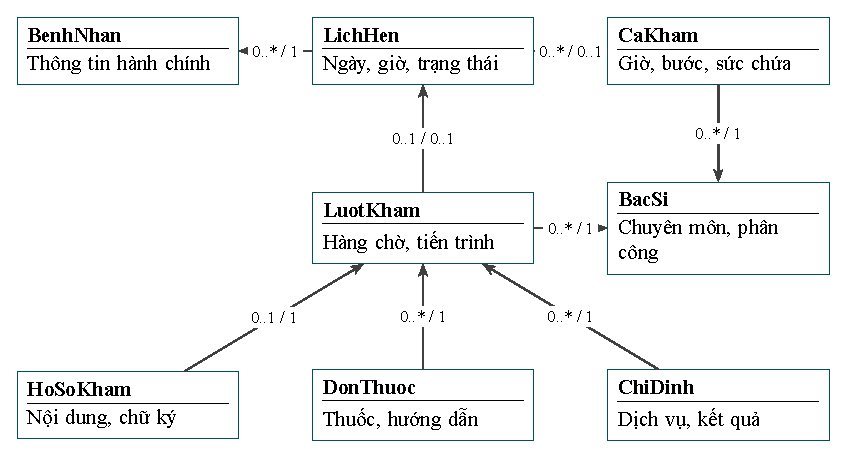
\includegraphics[width=1\textwidth,height=.61\textheight,keepaspectratio]{figures/diagrams/domain_care.pdf}\captionof{figure}{Mô hình lĩnh vực:\allowbreak{} người bệnh và chăm sóc}\label{fig:domain_care}\end{center}
Mô hình chọn các quan hệ trọng tâm; không phải ERD đầy đủ.\allowbreak{} Ký hiệu bội số ghi ở nhãn theo thứ tự nguồn/\allowbreak{}đích.\allowbreak{} Lượt vãng lai không bắt buộc có lịch hẹn, còn lịch chưa đến khám chưa có lượt.\allowbreak{} Hồ sơ và các chứng từ chuyên môn gắn lượt để tránh đồng nhất việc đặt với việc đã được phục vụ.\allowbreak{}

\clearpage

\Needspace{6\baselineskip}\subsection{Mô hình lĩnh vực:\allowbreak{} tài chính, dược và nhân sự}
\begin{center}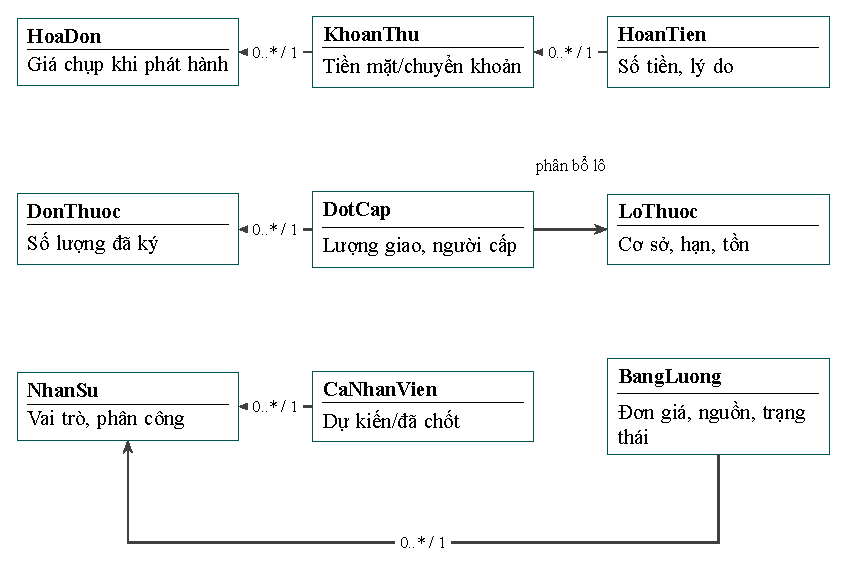
\includegraphics[width=1\textwidth,height=.61\textheight,keepaspectratio]{figures/diagrams/domain_ops.pdf}\captionof{figure}{Mô hình lĩnh vực:\allowbreak{} tài chính, dược và nhân sự}\label{fig:domain_ops}\end{center}
Khoản thu và hoàn tiền là các chứng từ bổ sung, không xóa hóa đơn.\allowbreak{} Quan hệ cấp phát-lô cần thực thể allocation để ghi nhiều lô cho một dòng đơn.\allowbreak{} Bảng lương lưu snapshot ca, không giữ một quan hệ trực tiếp bắt buộc tới từng ca nguồn trong khóa ngoại.\allowbreak{}

\clearpage

\section{Phân tích tương tác và quy trình}

\Needspace{6\baselineskip}\subsection{Tuần tự phân tích:\allowbreak{} hủy lịch có ngưỡng thời gian}
\begin{center}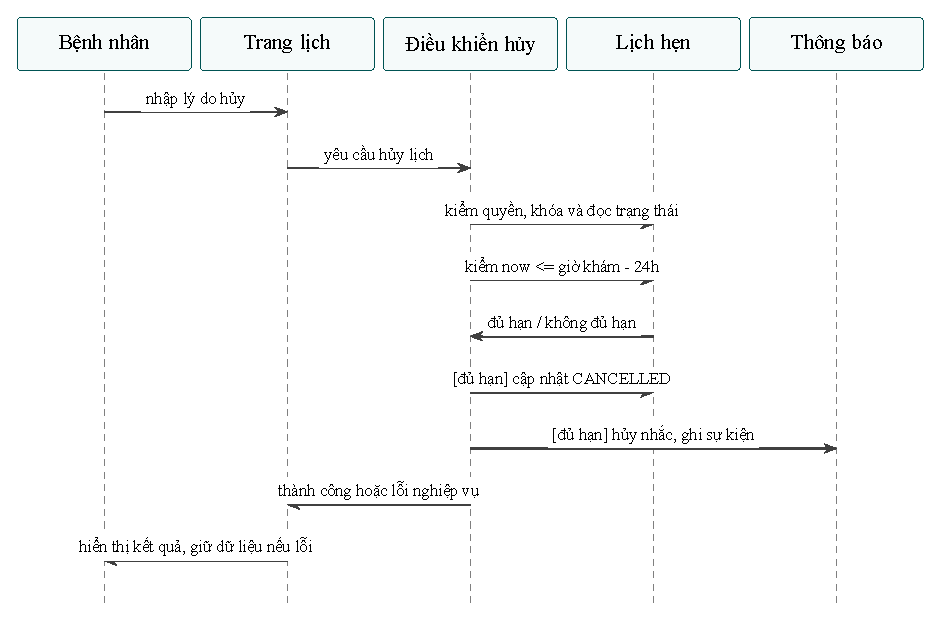
\includegraphics[width=1\textwidth,height=.61\textheight,keepaspectratio]{figures/diagrams/seq_cancel.pdf}\captionof{figure}{Tuần tự phân tích:\allowbreak{} hủy lịch có ngưỡng thời gian}\label{fig:seq_cancel}\end{center}
Sơ đồ ở mức phân tích thể hiện quyết định nghiệp vụ, không phải hai nhánh cùng được chạy.\allowbreak{} Khi không đủ hạn, không cập nhật lịch, không tạo lịch sử hay job mới.\allowbreak{} Đúng 24 giờ thuộc nhánh cho phép.\allowbreak{}

\clearpage

\Needspace{6\baselineskip}\subsection{Tuần tự phân tích:\allowbreak{} điều chỉnh hồ sơ đã ký}
\begin{center}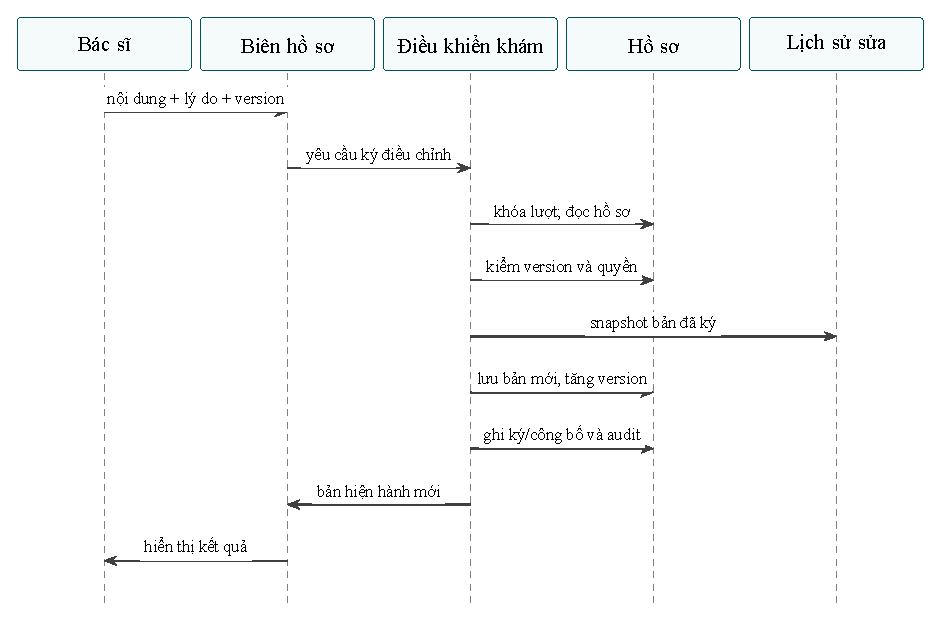
\includegraphics[width=1\textwidth,height=.61\textheight,keepaspectratio]{figures/diagrams/seq_record.pdf}\captionof{figure}{Tuần tự phân tích:\allowbreak{} điều chỉnh hồ sơ đã ký}\label{fig:seq_record}\end{center}
Trường hợp version không khớp dừng trước snapshot và cập nhật.\allowbreak{} Chỉ bác sĩ phụ trách đủ quyền mới thực hiện được; lý do điều chỉnh là dữ liệu nghiệp vụ bắt buộc, không chỉ là ghi chú tùy chọn trên giao diện.\allowbreak{}

\clearpage

\Needspace{6\baselineskip}\subsection{Tuần tự phân tích:\allowbreak{} xếp và chốt lịch nhân viên}
\begin{center}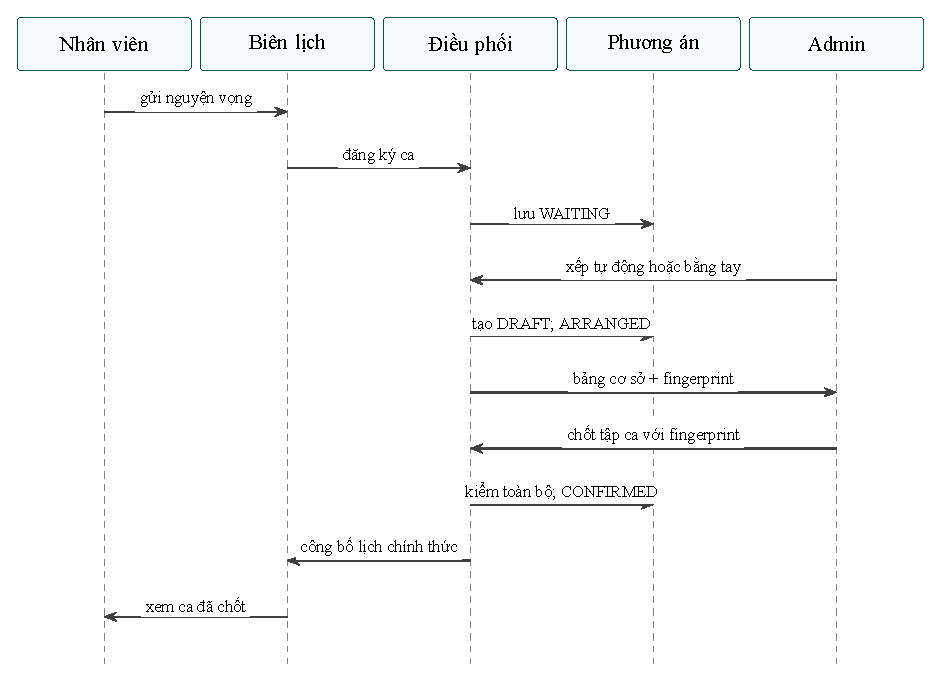
\includegraphics[width=1\textwidth,height=.61\textheight,keepaspectratio]{figures/diagrams/seq_roster.pdf}\captionof{figure}{Tuần tự phân tích:\allowbreak{} xếp và chốt lịch nhân viên}\label{fig:seq_roster}\end{center}
Đăng ký và phương án có trạng thái riêng.\allowbreak{} Admin rà soát trước chốt.\allowbreak{} Nếu fingerprint cũ hoặc một nhân viên không còn đủ điều kiện, không công bố một phần; lịch lâm sàng bác sĩ được giữ tách khỏi staff roster.\allowbreak{}

\clearpage

\Needspace{6\baselineskip}\subsection{Tuần tự phân tích:\allowbreak{} nhận thông điệp tích hợp}
\begin{center}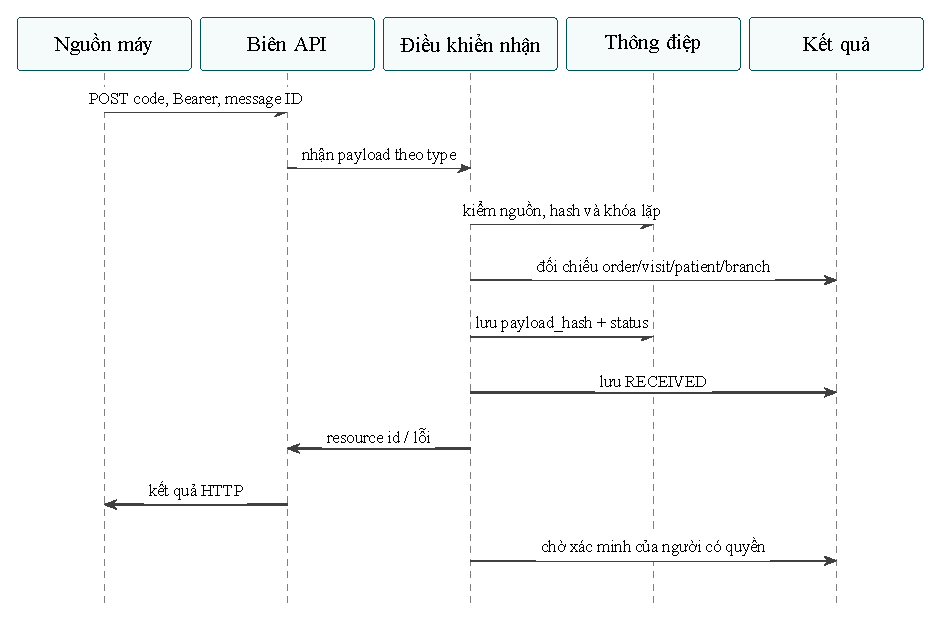
\includegraphics[width=1\textwidth,height=.61\textheight,keepaspectratio]{figures/diagrams/seq_integration.pdf}\captionof{figure}{Tuần tự phân tích:\allowbreak{} nhận thông điệp tích hợp}\label{fig:seq_integration}\end{center}
Thông điệp trùng phải có cùng nội dung mới được trả tài nguyên cũ.\allowbreak{} Nguồn máy không tự đặt kết quả VERIFIED.\allowbreak{} Sơ đồ mô tả mô hình mock nhận dữ liệu; chưa có adapter gửi chỉ định ra LIS ngoài.\allowbreak{}

\clearpage

\Needspace{6\baselineskip}\subsection{Hoạt động:\allowbreak{} từ đặt hẹn đến hoàn tất khám}
\begin{center}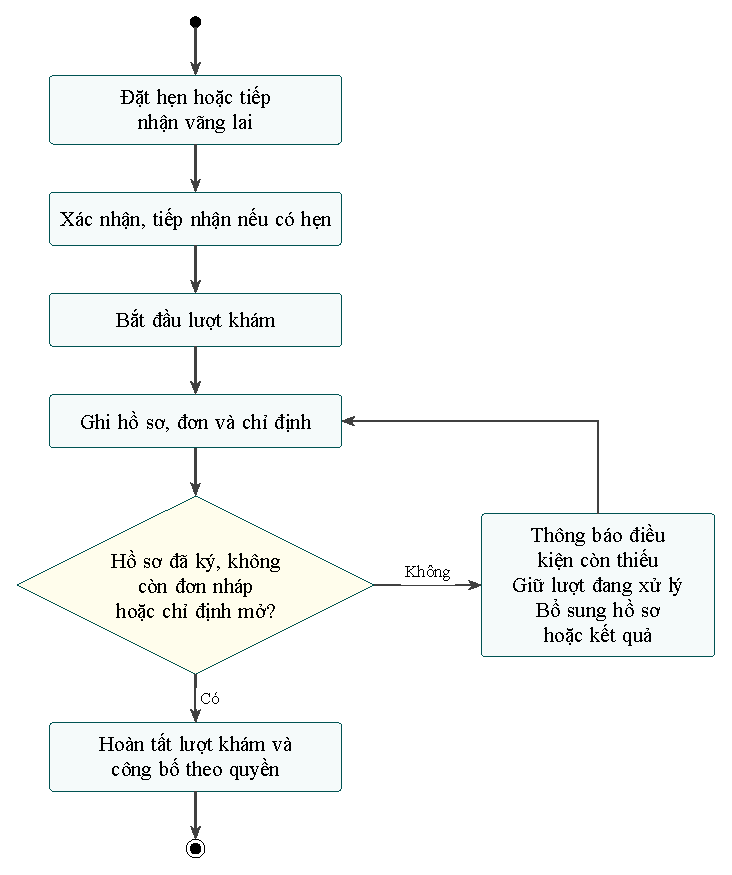
\includegraphics[width=1\textwidth,height=.61\textheight,keepaspectratio]{figures/diagrams/act_care.pdf}\captionof{figure}{Hoạt động:\allowbreak{} từ đặt hẹn đến hoàn tất khám}\label{fig:act_care}\end{center}
Người bệnh vãng lai được tiếp nhận trực tiếp mà không cần đặt hẹn.\allowbreak{} Khi chưa đủ điều kiện hoàn tất, lượt khám tiếp tục ở trạng thái đang xử lý để bổ sung hồ sơ, đơn thuốc hoặc kết quả.\allowbreak{} Sau bước hoàn tất, thu ngân và nhân sự cấp phát thực hiện các nghiệp vụ tiếp theo trong phạm vi quyền được cấp.\allowbreak{}

\clearpage

\Needspace{6\baselineskip}\subsection{Hoạt động:\allowbreak{} đăng ký, xếp và chốt lịch nhân viên}
\begin{center}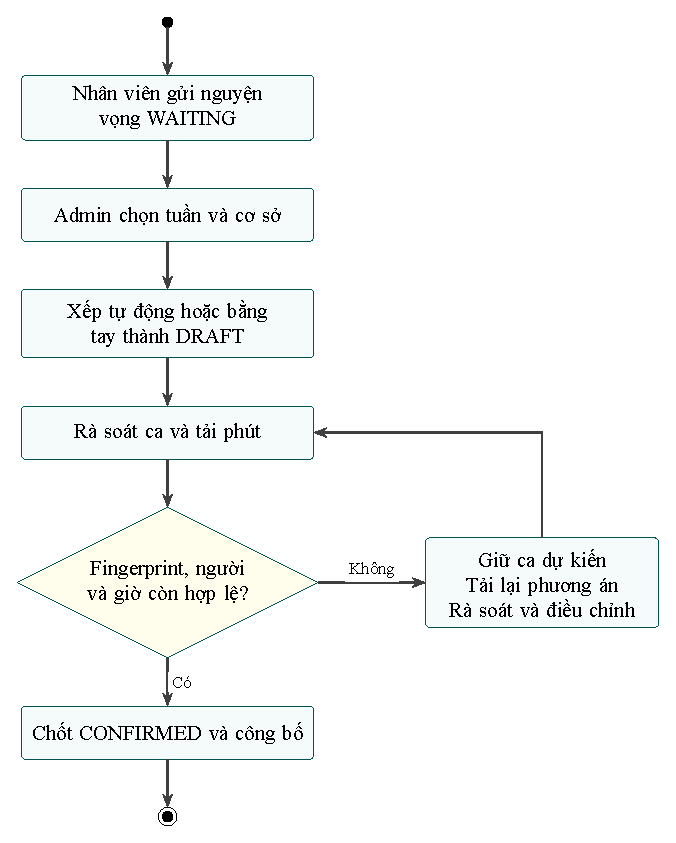
\includegraphics[width=1\textwidth,height=.61\textheight,keepaspectratio]{figures/diagrams/act_roster.pdf}\captionof{figure}{Hoạt động:\allowbreak{} đăng ký, xếp và chốt lịch nhân viên}\label{fig:act_roster}\end{center}
Lưu nguyện vọng không có nghĩa ca chính thức.\allowbreak{} Nhánh lỗi khi chốt giữ nguyên các ca dự kiến; người quản trị phải tải lại hoặc sửa điều kiện trước khi chốt.\allowbreak{} Bảng theo cơ sở giúp nhìn thiếu nhân sự nhưng phạm vi thao tác vẫn kiểm tại server.\allowbreak{}

\clearpage

\Needspace{6\baselineskip}\subsection{Hoạt động:\allowbreak{} phân bổ FEFO và rollback}
\begin{center}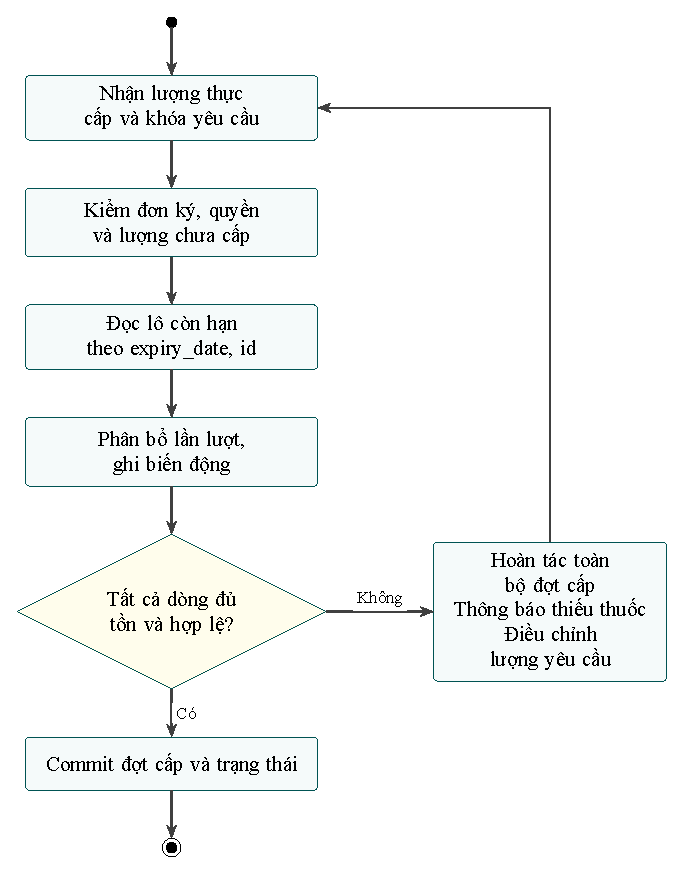
\includegraphics[width=1\textwidth,height=.61\textheight,keepaspectratio]{figures/diagrams/act_dispense.pdf}\captionof{figure}{Hoạt động:\allowbreak{} phân bổ FEFO và rollback}\label{fig:act_dispense}\end{center}
Các lần giảm ở trước điểm quyết định vẫn nằm trong transaction.\allowbreak{} Khi thiếu, nhánh lỗi rollback toàn bộ thay vì cấp một phần âm thầm.\allowbreak{} Nếu muốn cấp một phần, người dùng gửi lượng thực cấp nhỏ hơn phù hợp và hệ thống lưu rõ đợt đó.\allowbreak{}

\clearpage

\Needspace{6\baselineskip}\subsection{Hoạt động:\allowbreak{} đối chiếu và ghi nhận trả lương}
\begin{center}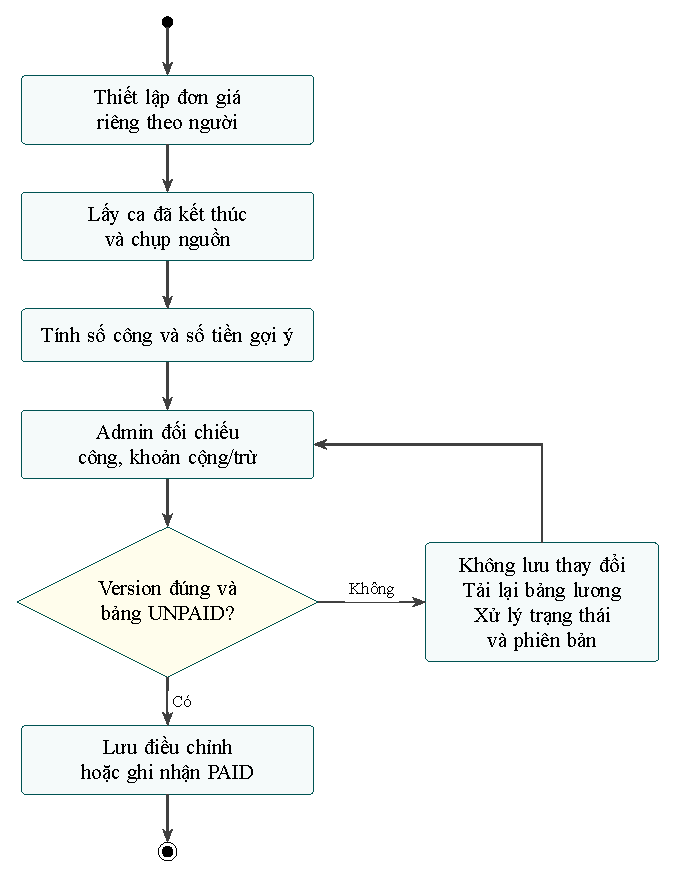
\includegraphics[width=1\textwidth,height=.61\textheight,keepaspectratio]{figures/diagrams/act_payroll.pdf}\captionof{figure}{Hoạt động:\allowbreak{} đối chiếu và ghi nhận trả lương}\label{fig:act_payroll}\end{center}
Chứng từ PAID khóa sửa tiền.\allowbreak{} Nếu cần sửa sau trả, admin mở về UNPAID có lý do trước.\allowbreak{} Nguồn giờ là lịch, nên đối chiếu thực tế là bước nghiệp vụ bắt buộc trước khi coi số tiền là khoản cần chi.\allowbreak{}

\clearpage

\section{Vòng đời và điều kiện chuyển trạng thái}

\Needspace{6\baselineskip}\subsection{Trạng thái lịch hẹn hiện hành}
\begin{center}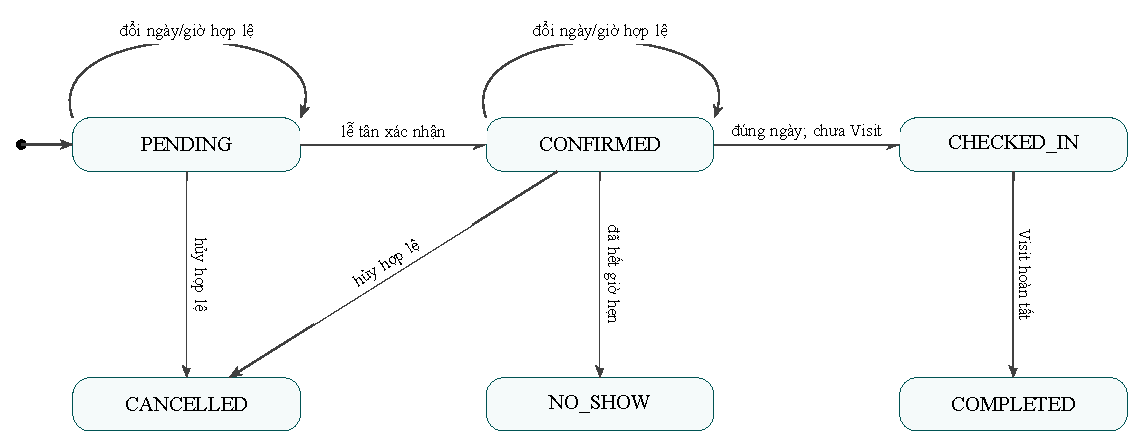
\includegraphics[width=1\textwidth,height=.61\textheight,keepaspectratio]{figures/diagrams/st_appointment.pdf}\captionof{figure}{Trạng thái lịch hẹn hiện hành}\label{fig:st_appointment}\end{center}
PENDING là chờ xác nhận; CONFIRMED là đã xác nhận.\allowbreak{} CHECKED\_\allowbreak{}IN đánh dấu đã tiếp nhận và tạo lượt khám.\allowbreak{} Quá trình khám được theo dõi riêng trên lượt khám.\allowbreak{} Đổi lịch hợp lệ giữ nguyên trạng thái PENDING hoặc CONFIRMED; hủy và vắng hẹn giải phóng chỗ đặt.\allowbreak{}

\clearpage

\Needspace{6\baselineskip}\subsection{Trạng thái lượt khám}
\begin{center}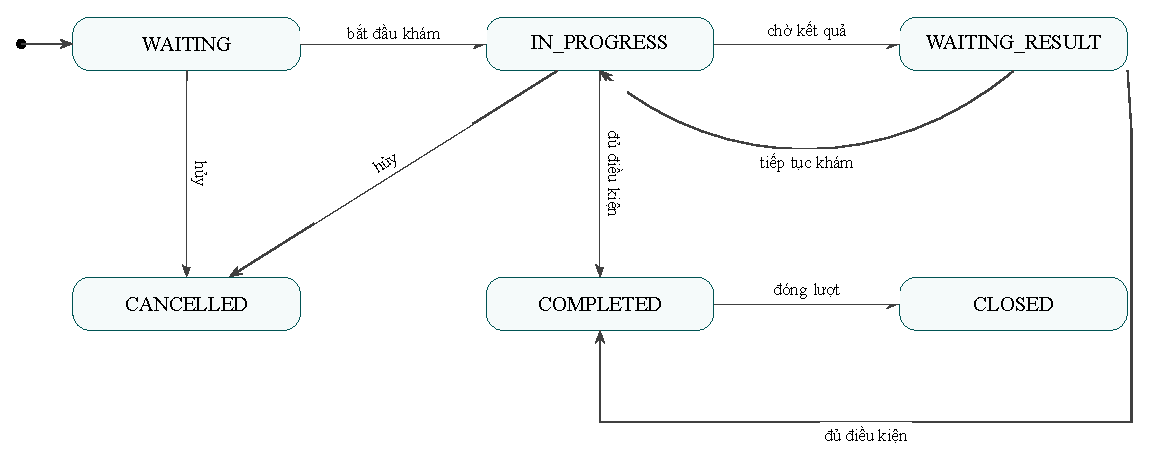
\includegraphics[width=1\textwidth,height=.61\textheight,keepaspectratio]{figures/diagrams/st_visit.pdf}\captionof{figure}{Trạng thái lượt khám}\label{fig:st_visit}\end{center}
Điều kiện COMPLETED được kiểm ở service:\allowbreak{} hồ sơ đã ký, không đơn nháp, không chỉ định chưa hoàn tất/\allowbreak{}hủy.\allowbreak{} Mốc started\_\allowbreak{}at chỉ ghi lần bắt đầu đầu tiên; completed\_\allowbreak{}at ghi lúc hoàn tất.\allowbreak{} Đóng lượt không cho tự sửa tự do, chỉ điều chỉnh hồ sơ ký theo quy trình.\allowbreak{}

\clearpage

\Needspace{6\baselineskip}\subsection{Trạng thái nguyện vọng nhân viên}
\begin{center}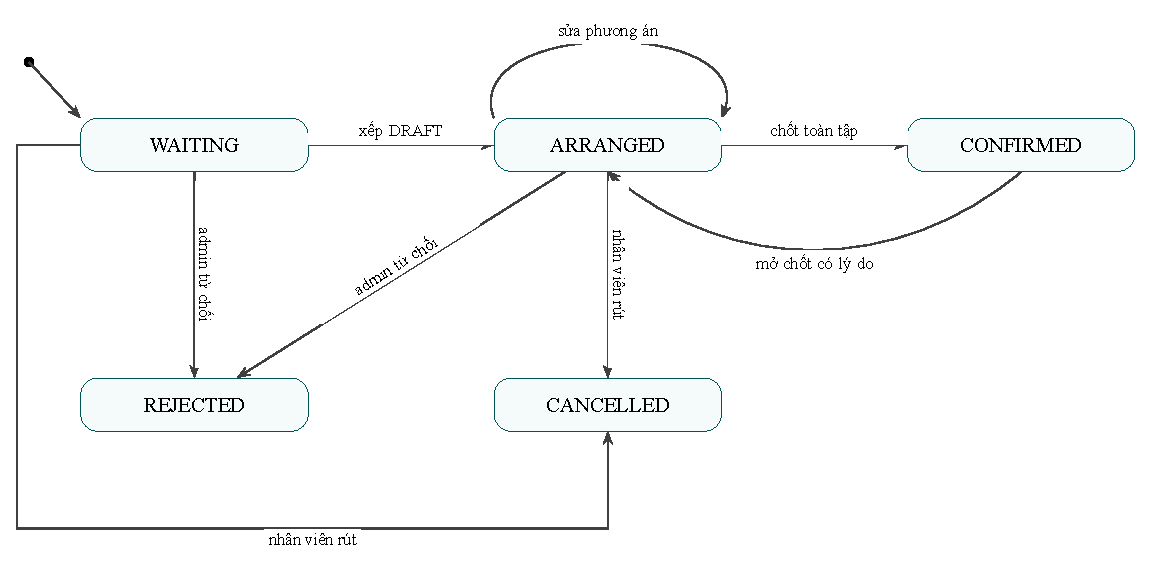
\includegraphics[width=1\textwidth,height=.61\textheight,keepaspectratio]{figures/diagrams/st_staff_request.pdf}\captionof{figure}{Trạng thái nguyện vọng nhân viên}\label{fig:st_staff_request}\end{center}
Đây là trạng thái request, không phải của Staff\allowbreak{}Work\allowbreak{}Shift.\allowbreak{} Ca tương ứng dùng DRAFT/\allowbreak{}CONFIRMED/\allowbreak{}CANCELLED.\allowbreak{} Rút hoặc từ chối ca chưa chốt hủy phương án liên quan; ca đã chốt phải được admin mở chốt trước khi điều chỉnh.\allowbreak{}

\clearpage

\Needspace{6\baselineskip}\subsection{Trạng thái yêu cầu chuyển ca bác sĩ}
\begin{center}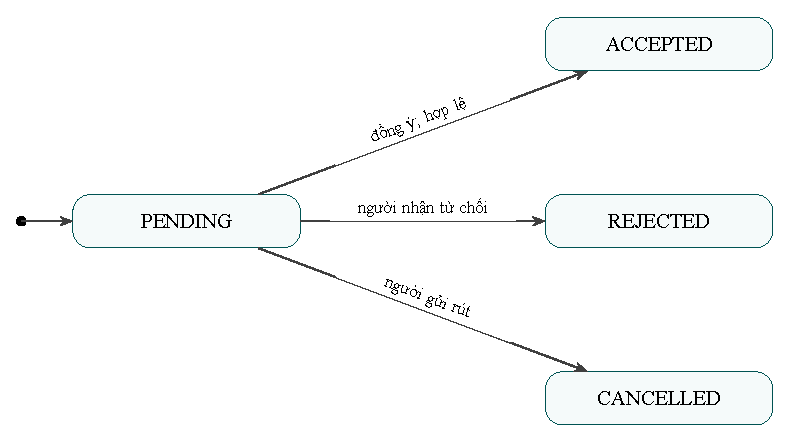
\includegraphics[width=1\textwidth,height=.61\textheight,keepaspectratio]{figures/diagrams/st_transfer.pdf}\captionof{figure}{Trạng thái yêu cầu chuyển ca bác sĩ}\label{fig:st_transfer}\end{center}
Yêu cầu chỉ được phản hồi khi đang PENDING và ca chưa bắt đầu.\allowbreak{} Khi chấp nhận, hệ thống kiểm tra lại chuyên môn, cơ sở và thời gian rảnh của người nhận, rồi chuyển ca cùng các lịch hẹn còn hiệu lực trong một giao dịch.\allowbreak{} Từ chối hoặc rút yêu cầu giữ nguyên người phụ trách.\allowbreak{}

\clearpage

\Needspace{6\baselineskip}\subsection{Trạng thái ghi nhận thanh toán lương}
\begin{center}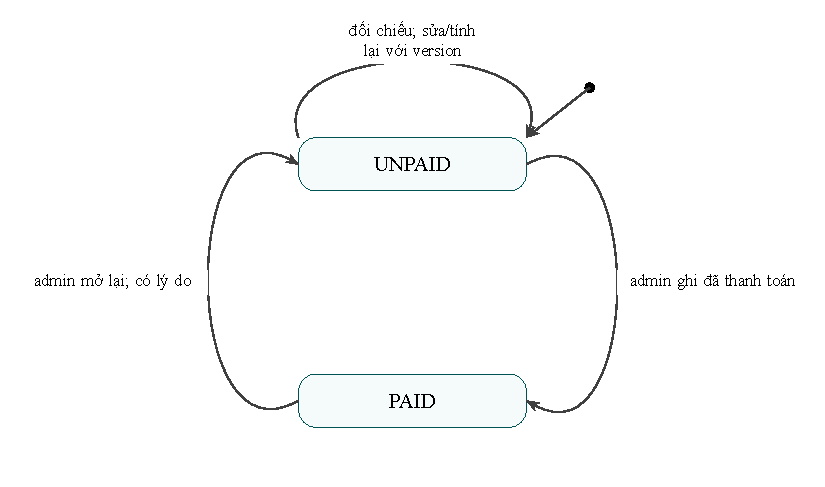
\includegraphics[width=1\textwidth,height=.61\textheight,keepaspectratio]{figures/diagrams/st_payroll.pdf}\captionof{figure}{Trạng thái ghi nhận thanh toán lương}\label{fig:st_payroll}\end{center}
Quản trị viên ghi nhận PAID sau khi đối soát chi trả ngoài hệ thống.\allowbreak{} Bảng đã thanh toán khóa các khoản tiền.\allowbreak{} Khi cần sửa, quản trị viên chuyển về UNPAID kèm lý do; hệ thống lưu dấu vết thay đổi trước khi cho phép điều chỉnh và ghi nhận chi trả lại.\allowbreak{}

